\documentclass[14pt]{article}
\usepackage[14pt]{extsizes}
\usepackage[utf8]{inputenc}
\usepackage[T2A]{fontenc}
\usepackage[english, russian]{babel}
\usepackage[a4paper,left=20mm, right=10mm, top=20mm, bottom=20mm]{geometry}
\usepackage{indentfirst, setspace}
\setlength{\parindent}{1.25cm}
\usepackage{tabularx, multirow}
\usepackage[normalem]{ulem}
\usepackage[style=russian]{csquotes}

\usepackage{graphicx}
\usepackage{wrapfig}
\graphicspath{ {images/} }

\fontsize{12}{12}\selectfont
\usepackage{amsmath,amsfonts,amssymb}
\usepackage{mathtools}
\usepackage{listings}
\usepackage[center]{caption}
\renewcommand{\labelenumii}{\arabic{enumi}.\arabic{enumii}.}
\renewcommand{\labelenumiii}{\arabic{enumi}.\arabic{enumii}.\arabic{enumiii}.}
\renewcommand{\labelenumiv}{\arabic{enumi}.\arabic{enumii}.\arabic{enumiii}.\arabic{enumiv}.}
\DeclareCaptionLabelSeparator{custom}{ --- }
\captionsetup{labelsep=custom}
\usepackage{pgfplots}
\usepackage{pdfpages}
\pgfplotsset{compat=1.9}
\usepackage{xcolor}
\usepackage{hyperref}
\definecolor{linkcolor}{HTML}{000000} 
\definecolor{urlcolor}{HTML}{000000} 
\hypersetup{pdfstartview=FitH,linkcolor=linkcolor,urlcolor=urlcolor, colorlinks=true}
\captionsetup[figure]{name=Рисунок}


\begin{document}
	
	{\centering
		\begin{bf}
			\begin{figure}[h]
				{\centering
					
\includegraphics[width=0.25\textwidth]{1}\par
				}
			\end{figure}
			
			
			\small{
				Министерство науки и высшего образования Российской Федерации\par
				Федеральное государственное\par
				бюджетное образовательное учреждение высшего образования\par
				\enquote{Московский государственный технический унверситет\par
					имени Н.Э. Баумана\par
					\hspace{2cm}(национальный исследовательский университет)}\par
				\hspace{2.0cm}(МГТУ им. Н.Э. Баумана)\par}
		\end{bf}
	}
	
	\vspace{0.5cm}
	
	{\setstretch{0.1}
		\noindent\rule{\textwidth}{1mm}
		\noindent\rule{\textwidth}{0.5mm}
		
	}
	
	\fontsize{14}{21}\selectfont
	
	\noindent\begin{tabularx}{\textwidth}{l >{\centering\arraybackslash}X}
		ФАКУЛЬТЕТ & \flqq Фундаментальные Науки\frqq \\ \cline{2-2}
		
		КАФЕДРА & ФН-12 \flqq Математическое моделирование\frqq \\ \cline{2-2}
	\end{tabularx}
	
	
	\vspace{1cm}
	
	
	\begin{center}
		\begin{bf}
			
			\fontsize{24}{36}\selectfont
			ОТЧЕТ
			
			\fontsize{20}{30}\selectfont
			ПО РУБЕЖНОМУ КОНТРОЛЮ №1 
			
			\fontsize{20}{30}\selectfont
			по дисциплине <<Типы и структуры данных>>
			
			Тема: <<Стек и очередь>>
			
		\end{bf}
	\end{center}
	
	\fontsize{14}{21}\selectfont
	\vspace{5cm}
	
	
	\noindent\begin{tabularx}{\textwidth}{ X >{\centering}p{4cm} p{1cm} c }
		Выполнил студент гр. ФН12-31Б: & & & Лямин И.С.\\ \cline{2-2} \cline{4-4}
		& \fontsize{10}{15}\selectfont дата, подпись & & \fontsize{10}{15}\selectfont Ф.И.О. \\
		Проверил преподаватель: & & & Волкова Л. Л.\\ \cline{2-2} \cline{4-4}
		& \fontsize{10}{15}\selectfont дата, подпись & & \fontsize{10}{15}\selectfont Ф.И.О.
	\end{tabularx}
	
	\vspace{\fill}
	
	\begin{center}
		\it{Москва}, 2024
	\end{center}
	
	\thispagestyle{empty} 
	
	\newpage
	\renewcommand{\contentsname}{\centering{СОДЕРЖАНИЕ}}
	\setcounter{page}{2}
	\tableofcontents
	
	\newpage
	\begin{center}
		\section*{ВВЕДЕНИЕ} 
	\end{center}
	
	В рубежном контроле будет реализовано две циклические структуры данных, циклическая очередь и стек.\\
	\textbf{Цель работы:} Реализовать структуры данных циклический стек, циклическую очередь и интерфейс взаимодействия с ними.
	Для достижения поставленной цели требуется выполнить следующие задачи.
	\begin{enumerate}
		\item Описать необходимые структуры данных.
		\item Реализовать структуры данных.
		\item Реализовать методы интерфейса для взаимодействия с СД.
	\end{enumerate}
	
	\newpage
	\section{Аналитическая часть}	
	\textbf{Стек} --- структура данных которая позволяет извлечь только последний помещённый в неё элемент (FILO - первый зашёл, последний вышел).
	
	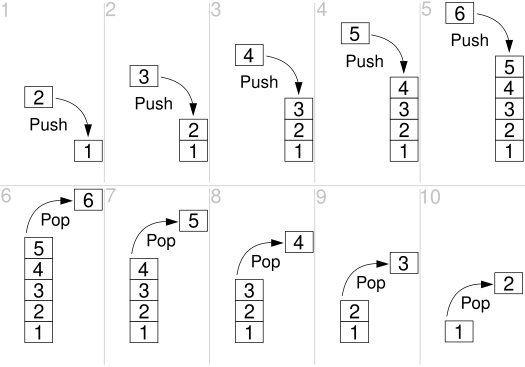
\includegraphics[width = 0.8\textwidth, height = 0.5\textheight]{Stack}
	\captionof{figure}{Cхема работы стека}
	\label{fig:label1}
	
	\textbf{Интерфейс стека}:
	\begin{enumerate}
		\item Push - добавление элемента в конец массива.
		\item Pop - удаление последнего элемента.
		\item IsFull - проверка на полноту.
		\item IsEmpty - проверка на пустоту.
		\item Leek - вывод в консоль массива изначального с индесами и пользовательского массива.
	\end{enumerate}
	
	\newpage
	\textbf{Циклическая очередь} --- это структура данных позволяющая извлеч только первый помешённый в неё элемент (FIFO - первый зашёл, первый вышел). Циклическая очередь от обычной отличается тем, что если при полном заполнении памяти удалить один элемент и попытаться поместить на его место новый помещённый на его место элемент будет первым только в изначальном массиве, отображаться он будет как последний.
	\begin{center}
		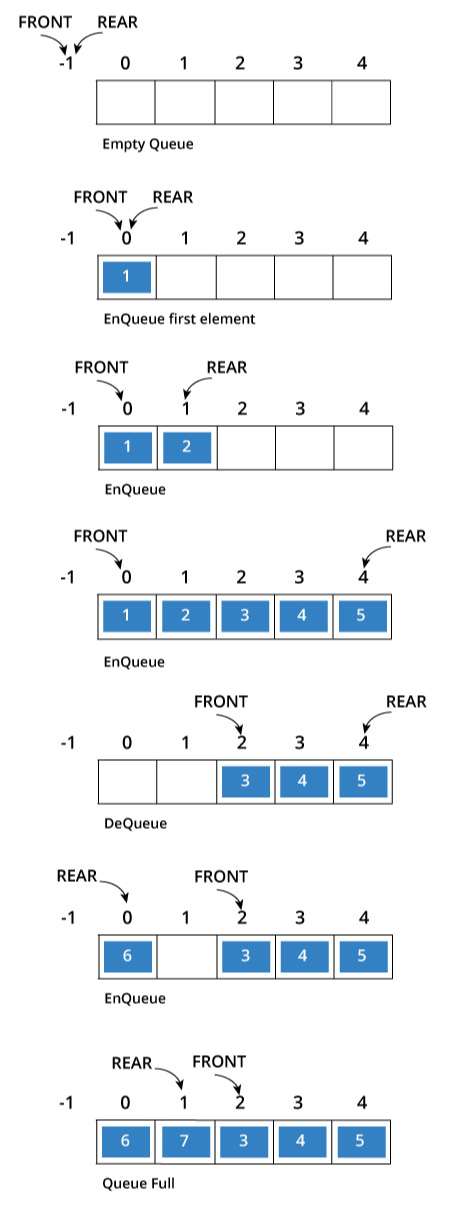
\includegraphics[width = 0.6\textwidth, height = 0.75\textheight]{Turn}
		\captionof{figure}{Cхема работы циклической очереди}
		\label{fig:label2}
	\end{center}
	\newpage
	\textbf{Интерфейс очереди}:
	\begin{enumerate}
		\item Push - добавление элемента в конец массива.
		\item Delete - удаление первого элемента.
		\item IsFull - проверка на полноту.
		\item IsEmpty - проверка на пустоту.
		\item Leek - вывод в консоль массива изначального с индесами и пользовательского массива.
	\end{enumerate}
	
	
	\newpage
	\section{Конструкторская часть}
	
	На рисунках~\ref{fig:label3}--\ref{fig:label8} представлены функциональнальные схемы функций, осуществляющих работу со стеком и очередью. Функциональные схемы даны в нотации IDEF0.
	
	\begin{center}
		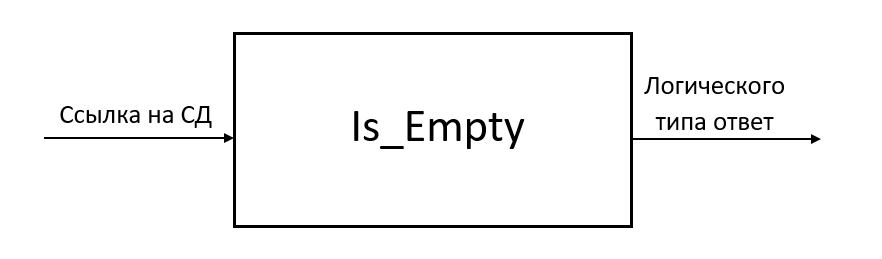
\includegraphics[width = 0.9\textwidth, height = 0.2\textheight]{is_empty}
		\captionof{figure}{Функция проверки на пустоту СД}
		\label{fig:label3}

		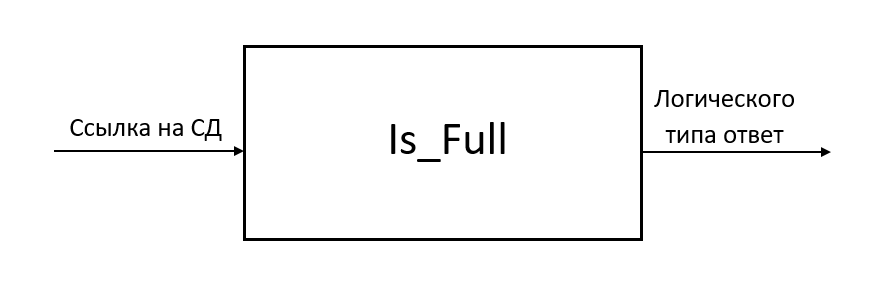
\includegraphics[width = 0.9\textwidth, height = 0.25\textheight]{is_full}
		\captionof{figure}{Функция проверки на полноту СД}
		\label{fig:label4}
		
		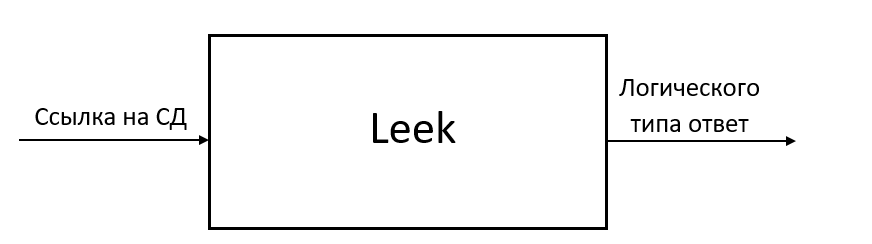
\includegraphics[width = 0.92\textwidth, height = 0.2\textheight]{leek}
		\captionof{figure}{Функция вывода информации о СД}
		\label{fig:label5}
		
		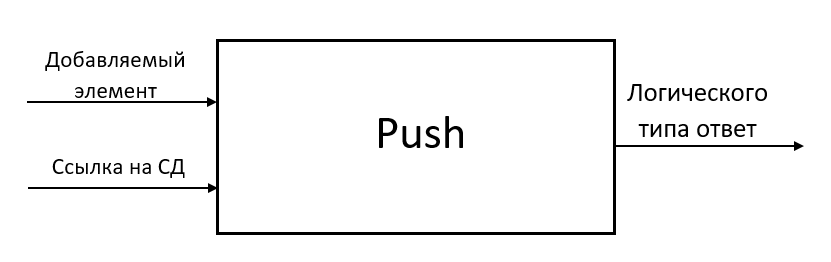
\includegraphics[width = 0.92\textwidth, height = 0.2\textheight]{push}
		\captionof{figure}{функция добавления элемента в конец СД}
		\label{fig:label6}
		
		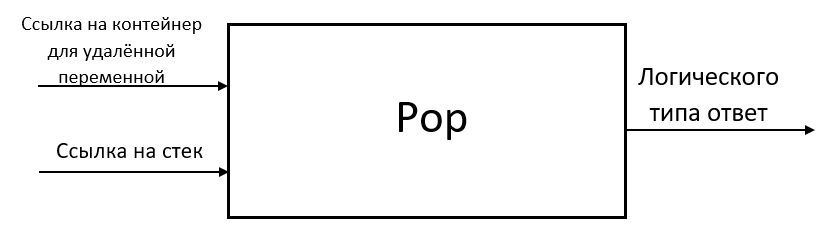
\includegraphics[width = 0.92\textwidth, height = 0.2\textheight]{pop (1)}
		\captionof{figure}{функция удаления последнего элемента из стека}
		\label{fig:label7}
		
		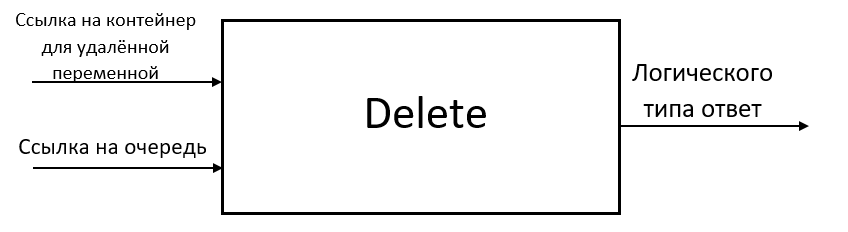
\includegraphics[width = 0.92\textwidth, height = 0.2\textheight]{delete}
		\captionof{figure}{функция удаления первого элемента из очереди}
		\label{fig:label8}
		
	\end{center}
	
	\newpage
	\par 
	
	\newpage
	
	\section{Технологическая часть} 
	
	\subsection{Выбор средств реализации}
	Для программной реализации СД использовалась среда разработки Visual Studio, язык программирования, на котором была выполнена реализации СД, --- C++. 
	Исследование проводилось на ноутбуке (64-разрядная операционная система, процессор x64, частота процессора 3.10~ГГц, оперативная память 16~ГБ)\par
	
	\subsection{Реализация СД}
	В листинге~\ref{list1} можно увидеть программную реализацию описанных СД.
	\lstset{
		language=C++,
		basicstyle=\ttfamily\fontsize{12}{14}\selectfont,
		breaklines=true,
		keywordstyle=\color{blue},
		commentstyle=\color{gray},
		stringstyle=\color{red},
		postbreak=\mbox{\textcolor{red}{$\hookrightarrow$}\space},
		showstringspaces=false,
		keepspaces=true,
		numbers=left,              
		numberstyle=\tiny,           
		stepnumber=1,                 
		numbersep=5pt,               
		backgroundcolor=\color{white},
		frame=single,  
	}
	
\begin{lstlisting}[label = list1, caption = Программная реализация]
struct Turn{
	int capacity = 0;
	int col_elem = 0;
	int array[SIZE];
	int start = 0;
	int end = 0;
	
	Turn(int capacity) {
		this->capacity = capacity;
		for (int i = 0; i < capacity; i++) {
			this->array[i] = -1;
		}
	}
};


struct Stack {
	int capacity = 0;
	int col_elem = 0;
	int array[SIZE];
	int end = 0;
	int start = 0;
	
	Stack(int capacity) {
		this->capacity = capacity;
		for (int i = 0; i < capacity; i++) {
			this->array[i] = -1;
		}
	}
};

template<typename DS>
bool IsEmpty(DS* turn) {
	if (turn->col_elem == 0) return true;
	return false;
}

bool Pop(Stack* stack, int* contain) {
	if (IsEmpty(stack)) return false;
	*contain = stack->array[stack->end];
	stack->array[stack->end] = -1;
	stack->end -= 1;
	cout << "Number " << (*contain) << " extracted from stack" << endl;
	stack->col_elem -= 1;
	return true;
}

template<typename DS>
bool IsFull(DS* turn) {
	if (turn->capacity == turn->col_elem) return true;
	return false;
}


bool Push(Turn* turn, int* elem) {
	if (IsFull(turn)) {
		cout << "Array is full" << endl;
		return 0;
	}
	int iter;
	for (int i = turn->start; i <= (turn->start + turn->capacity - 1); i++) {
		iter  = i % turn->capacity;
		if (turn->array[iter] == -1) {
			if (IsEmpty(turn)) {
				cout << "Stack was empty" << endl;
				turn->col_elem += 1;
				turn->start = iter;
				turn->end = iter;
				turn->array[iter] = (*elem);
				return 1;
			}
			cout << "Stack was NOT empty" << endl;
			turn->col_elem += 1;
			turn->end = iter;
			turn->array[iter] = (*elem);
			return 1;
		}
	}
	return 0;
}

bool Push_stack(Stack* turn, int* elem) {
	if (IsFull(turn)) {
		cout << "Array is full" << endl;
		return 0;
	}
	int iter;
	for (int i = 0; i < turn->capacity; i++) {
		if (turn->array[i] == -1) {
			if (IsEmpty(turn)) {
				cout << "Stack was empty" << endl;
				turn->col_elem += 1;
				turn->end = i;
				turn->array[i] = (*elem);
				return 1;
			}
			cout << "Stack was NOT empty" << endl;
			turn->col_elem += 1;
			turn->end = i;
			turn->array[i] = (*elem);
			return 1;
		}
	}
	return 0;
}

bool Delete(Turn* turn, int* contain){
	if (IsEmpty(turn)) return false;
	if (turn->start == turn->end) {
		*contain = turn->array[turn->start];
		turn->array[turn->start] = -1;
		turn->start = 0;
		turn->end = 0;
		cout << "Number " << (*contain) << " extracted from stack, stack is now empty" << endl;
		turn->col_elem -= 1;
		return true;
	}
	*contain = turn->array[turn->start];
	turn->array[turn->start] = -1;
	turn->start = ((turn->start + 1) % turn->capacity);
	cout << "Number " << (*contain) << " extracted from stack" << endl;
	turn->col_elem -= 1;
	return true;
}

template<typename DS_2>
void print_basic_array(DS_2* turn) {
	for (int i = 0; i < turn->capacity; i++) {
		if ((i == turn->start) && (i == turn->end)) {
			cout << turn->array[i] << " --- BOTH" << endl;
			continue;
		}
		try
		{
			if (i == turn->start) {
				cout << turn->array[i] << " --- START" << endl;
				continue;
			}
		}
		catch (const std::exception&)
		{
			cout << "";
		}
		if (i == turn->end) {
			cout << turn->array[i] << " --- END" << endl;
			continue;
		}
		cout << turn->array[i] << endl;
	}
	cout << turn->col_elem << " --- elemnts" << endl;
}

template<typename DS_2>
void print(DS_2* turn) {
	int colis = 0;
	for (int i = 0; i < (turn->capacity); i++) {
		int ind = (i + turn->start) % turn->capacity;
		if (turn->array[ind] == -1) {
			colis += 1;
			continue;
		}
		cout << "[" << i - colis << "]" << " --- " << turn->array[ind] << endl;   
	}
	cout << turn->col_elem << " --- elemnts" << endl;
}

void read(int* number) {
	cout << "Input a nubmer: ";
	
	while (true) {
		cin >> (*number);
		if (cin.fail()) {
			cin.clear(); 				cin.ignore(numeric_limits<streamsize>::max(), '\n'); 
			cout << "Error! Please, input a valid number: ";
		}
		else {
			break; 
		}
	}
}
\end{lstlisting}
	
	\section{Исследовательская часть}
	\subsection{Тестирование программы}
В таблицах~\ref{tab:tests} представлены описания тестов по методологии чёрного ящика, все тесты пройдены успешно.
	\begin{table}[htbp]
		\centering
		\begin{tabular}{|p{0.05\linewidth}|p{0.2\linewidth}|p{0.12\linewidth}|p{0.25\linewidth}|p{0.25\linewidth}|}
			\hline
			& \textbf{Описание теста} & \textbf{Входные данные} & \textbf{Ожидаемый результат} & \textbf{Полученный результат} \\
			\hline
			
			\textbf{1} & проверка на обработку не валидных данных & 3 & оповещение о некорректности данных и запрос новых & оповещение о некорректности данных и запрос новых \\
			\hline
			
			\textbf{2} & проверка на обработку не валидных данных & 1 -1&оповещение программы и запрос новых данных&оповещение программы и запрос новых данных\\
			\hline
			
			\textbf{3} & работа очереди & 2 \newline 3\newline 
			1\newline 2\newline 3 \newline Delete \newline Push \newline 10 \newline IsEmpty \newline IsFull & 10-end \newline 2-start \newline 3 \newline No it's not empty \newline Yes it's full
			& 10-end \newline 2-start \newline 3 \newline No it's not empty \newline Yes it's full\\
			\hline
			
			\textbf{4} & работа стека & 2\newline 
			3\newline 1\newline 2 \newline 3 \newline Pop \newline Push \newline 10 \newline IsEmpty \newline IsFull & 2-start \newline 2 \newline 10-end \newline  No it's not empty \newline Yes it's full & 2-start \newline 2 \newline 10-end \newline  No it's not empty \newline Yes it's full\\
			\hline
			
		\end{tabular}
		\caption{}
		\label{tab:tests}
	\end{table}	
	
	
	\newpage
	
	\section*{ЗАКЛЮЧЕНИЕ}	
	В результате лабораторной работы была достигнута цель - рассмотрены и разобраны две СД (циклическая очередь, стек).
	Были выполнены все поставленные задачи:
	\begin{enumerate}
		\item Описаны необходимые структуры данных.
		\item Реализованны структуры данных.
		\item Реализованы методы интерфейса для взаимодействия с СД.
	\end{enumerate}
	
	\newpage
	\begin{center}
		\section*{СПИСОК ИСПОЛЬЗОВАННЫХ ИСТОЧНИКОВ} 
		\addcontentsline{toc}{section}{СПИСОК ИСПОЛЬЗОВАННЫХ ИСТОЧНИКОВ}
	\end{center}
	\begin{enumerate}
		\item Т.Кормен, Ч.Лейзерсон, Р.Ривест, К.Штайн - Алгоритмы.\label{s:1}
		\item evileg.com [Электронный ресурс] -\par 
		URL:https://evileg.com/ru/post/472/\par
		(дата обращения: 25.09.2024).\label{s:2}
	\end{enumerate}
	
\end{document}

